\chapter{成为空间管理大师}
\label{cha:manage-storage}

\begin{intro}
  本章会为大家在用电脑时非常苦恼的一件事——硬盘空间吃紧,来提供一些建议与小技巧,看完本章,下面的问题你应该有了眉目:
  \begin{itemize}
    \item 为什么我的 C 盘不知不觉就红了?C 盘要多大才合适?
    \item 分区快满了(「红了」)怎么办?
    \item 我怎么把我的某个分区扩大/缩小一点?
    \item 有没有什么办法把 C 盘一些占空间又不能动的东西移到别处去?
  \end{itemize}
\end{intro}

在正式进入这一章之前,请大声朗读三遍以下八字真言,并时刻牢记于心:
\begin{center}
  \LARGE\bfseries
  数据无价,谨慎操作!\par
  Data is Precious, Operate Carefully!
\end{center}

如果要给「常见电脑问题」列个榜单,除了「软件怎么不能用」「为什么电脑变慢了」这种笼统的问题外,「我电脑又满了」肯定榜上有名。「满」,大部分指的是系统分区 C 盘。本章的所有内容,正是围绕「怎么样让我的电脑不那么满」这一需求展开的。

\section{谁「吃」了我的 C 盘?}

早年间,大约到 Windows 7 时代为止,C 盘空间大小并没有今天这般令人苦恼。彼时的日常用户,为 C 盘提供约 60 GB 空间,就能满足这台电脑以后一直使用的需求。Windows 8 系列暂且不论(反正也没多少人用),自 Windows 10 时代开始,系统本身与后续使用对空间的需求似乎迅速提升了。人们想着:「大概为 C 盘分个 100 GB 应该差不多吧。」然而事与愿违,如此想法总是导致了这样的事情:

\begin{figure}[htb!]
  \centering
  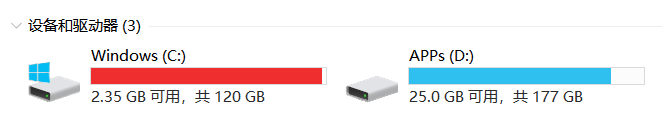
\includegraphics[width=.8\textwidth]{assets/advanced/Red_C_Drive.png}
  \caption{《红盘》}
  \label{fig:Red_C_Drive}
\end{figure}

但是,系统在初装时只占用了 20 至 30 GB 不等的空间,而即使我们将软件尽量装到其他分区中,为何用着用着 C 盘还是变成「红盘」了呢?这是因为软件所占的空间不止是本体,还有它在运行期间所产生的各种数据。

\begin{figure}[htb!]
  \centering
  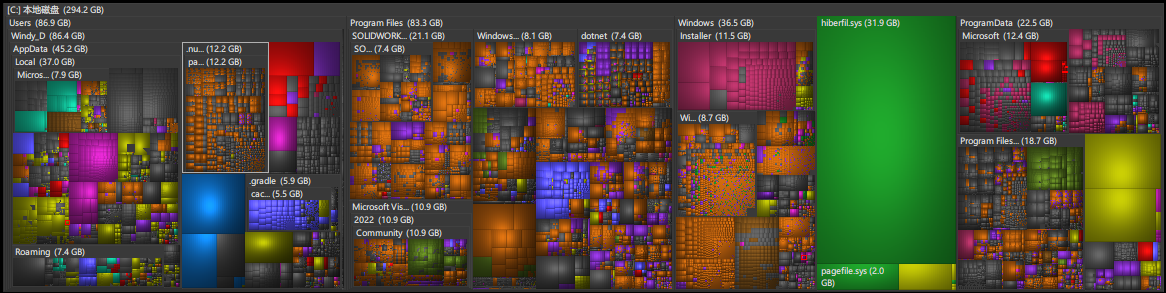
\includegraphics[width=.9\textwidth]{assets/advanced/Scan_C_Drive.png}
  \caption{C 盘的 WizTree 扫描结果}
  \label{fig:Scan_C_Drive}
\end{figure}

用 WizTree 分析一下 C 盘(详见\chapref{cha:tools-software}),你可能会发现,占空间最多的部分,除了系统文件夹 \MissingVerb{Windows} 以外,还有应用程序相关的文件夹(\MissingVerb{Program Files}、\MissingVerb{Program Files (x86)},以及 \MissingVerb{Program Data})、你自己的用户文件夹,以及两个神秘的 \MissingVerb{hiberfil.sys} 和 \MissingVerb{pagefile.sys} 文件。让我们来一一探查它们。

\subsection{程序文件夹}

你如果留心观察过软件的安装过程,或者仔细阅读了\chapref{cha:software-installation}一章,就会知道 \MissingVerb{Program Files} 与 \MissingVerb{Program Files (x86)} 两个文件夹是用来存放软件本体的文件夹。不过,实际上它们存放的是「为所有用户安装的软件」,至于只为单个用户安装的软件,我们后面再说。那么,为什么要分两个文件夹呢?

目前,我们所使用的几乎所有电脑都使用「64 位」的 CPU,运行「64 位」的操作系统。目前,多数软件也都是 64 位的。然而,由于某些历史原因,仍然有不少的应用软件是 32 位的,但 64 位电脑也能够兼容运行。操作系统为了分开管理不同位数的软件,划出了两个软件文件夹,\MissingVerb{Program Files} 用来存放 64 位的软件,而 \MissingVerb{Program Files (x86)} 存放 32 位的。

\begin{note}
  有关这 32 位和 64 位的本质、由来和历史,请参见\chapref{cha:program-and-arch}。
\end{note}

至于 \MissingVerb{Program Data} 文件夹,平时它的存在感似乎微乎其微,毕竟它是一个隐藏文件夹。启用「显示隐藏文件」选项,你就可以在 C 盘根目录看到它。这个文件夹的作用,顾名思义,用来存放应用程序的数据。但是这里还要加上一些限定词,是用来存放「适用于所有用户」的数据。所以,\regcolor{即便你选择把软件安装到了别的分区,它仍然可能在使用过程中往 C 盘放东西}。

在\chapref{cha:user-and-ms-account}中我们知道了「多用户」的事情,而这 \MissingVerb{Program Data} 文件夹存放的数据是不随用户变化而变化的「全局数据」。那用户自己特定的数据呢?这个问题的答案呼之欲出。

\subsection{用户文件夹}

用户文件夹里面的内容,我们一般见得多的,就是「桌面」「文档」「下载」这几个在资源管理器左侧可以看见的「已知文件夹」。但即便你不往这里面塞东西,你的用户文件夹还是可能非常庞大,毕竟,\regcolor{不只有你自己会往用户文件夹塞东西}。

首先打开 \MissingVerb{文档} 文件夹,里面可能会有一些以软件名称或软件开发商名称命名的文件夹。这些文件夹正是那些软件存放用户文件的地方,例如一些游戏的存档,软件保存的文档、工程文件等等。这些是软件认为你用得着的数据。

再打开你的用户文件夹,它位于 \MissingVerb{C:\用户\<你的用户名>},这里有一个隐藏的 \MissingVerb{AppData} 文件夹,是存放所有软件用于你这个用户的数据,整个用户文件夹中「看不见的内容」大多都在这里面。它里面有三个子文件夹:
\begin{itemize}
  \item \MissingVerb{Roaming}:意为「漫游」,如果你在别的电脑上登录了相同账户,那么这部分内容会同步过去;
  \item \MissingVerb{Local}:意为「本地」,这个文件夹一般是三个中最大的,存放那些「只为当前用户安装的软件本体」与「当前账户本地使用的所有软件数据」,不会同步;
  \item \MissingVerb{LocalLow}:意为「本地低权限」,软件处于类似「受限模式」下可以访问的数据(例如浏览器的无痕模式),里面内容最少,也不会同步。
\end{itemize}

值得一提的是,Windows 中定义了几个「环境变量」指向这些文件夹:\MissingVerb 指向上述 \MissingVerb{Roaming} 文件夹、\MissingVerb 则是 \MissingVerb{Local} 文件夹。大部分时候,这些环境变量可替代它们的真实路径来使用:按下 \keys{\Windows + R},或直接在资源管理器的地址栏内输入这些环境变量,就能进入这些文件夹。

\begin{figure}[htb!]
  \centering
  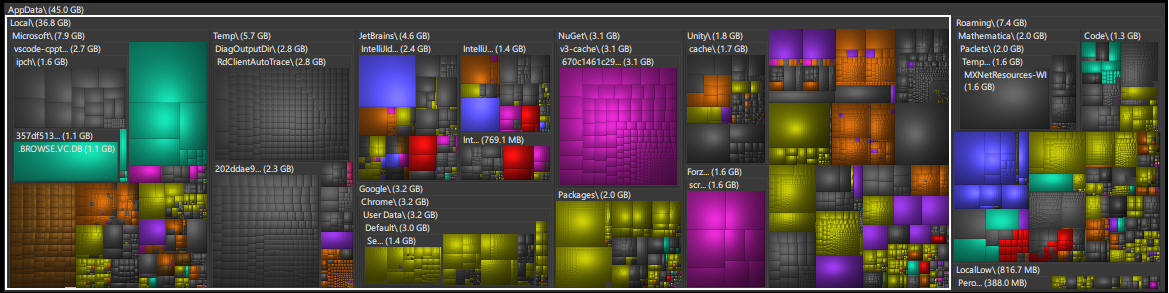
\includegraphics[width=.9\textwidth]{assets/advanced/AppData.png}
  \cprotect\caption{\MissingVerb{Appdata} 文件夹的 WizTree 扫描结果}
  \label{fig:AppData}
\end{figure}

\MissingVerb{AppData} 文件夹一般不能乱动,软件通常会自己管理里面的内容。如果你对自己没有十足的信心,移动、删除里面的内容很有可能造成软件工作异常。不到万不得已的时候,不要考虑动它。

\begin{figure}[htb!]
  \centering
  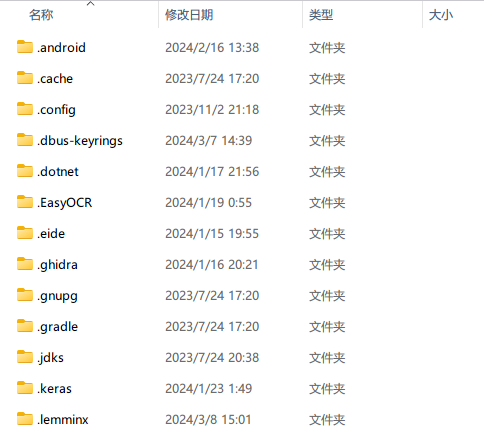
\includegraphics[width=.55\textwidth]{assets/advanced/Dev_Tool_Files.png}
  \cprotect\caption{用户文件夹中 \MissingVerb{.} 开头的目录}
  \label{fig:Dev_Tool_Files}
\end{figure}

此外,如果你是开发人员,装了许许多多软件开发工具,那么打开用户文件夹时映入眼帘的很可能会是一大列以 \MissingVerb{.} 开头的文件夹。这些文件夹多是不同开发工具放在这里的数据,包括但不限于软件包、SDK、插件等等内容,这些也占据了相当一部分的空间。

\subsection{页面文件和休眠文件}

在 WizTree 的分析页面中,我们往往可以看见两个奇怪的巨大文件:\MissingVerb{pagefile.sys} 和 \MissingVerb{hiberfil.sys}。它们有时可以占据十几甚至是几十 GB 的 C 盘空间,如下图所示。它们的真名是「页面文件」和「休眠文件」,是 Windows 系统运行所需要的。

\begin{figure}[htb!]
  \centering
  \vspace*{-.2cm}
  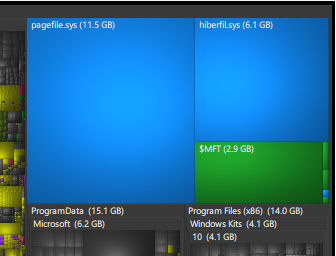
\includegraphics[width=6cm]{assets/advanced/Pagefile_and_hiberfil.png}
  \caption{WizTree 中展示的页面文件和休眠文件}
\end{figure}

页面文件的作用,是给系统提供「虚拟内存」:当电脑的内存不足以容纳打开的全部软件时,操作系统会将内存中暂时未用到的一部分数据存入硬盘,从而腾出空间给正在使用的数据和程序。而当我们需要用到那些被存入硬盘的数据时,操作系统再将它们取回内存,同时从内存中取出另一部分近期未用的数据换入硬盘。由于这个交换以一定大小的「页」为单位,硬盘中负责暂存内存数据的文件就称为「页面文件」。在 Windows 系统中,页面文件的默认位置就是 \MissingTT{C:\textbackslash{}pagefile.sys} (系统级隐藏,所以看不见)。它的大小因机器的内存而异,从几 GB 到几十 GB 都有可能。

而休眠文件的作用同样与内存有关。「休眠」(Hibernate)是电脑的一种工作状态,全机断电,但是上电后可以快速恢复到休眠前的状态。由于内存断电就丢失数据的特性,当需要休眠时,操作系统要先将内存里的数据全部存入硬盘——放在这休眠文件中。休眠文件默认位于 \MissingVerb{C:\hiberfil.sys},同样也是系统级隐藏的,在资源管理器中看不见它。它的默认大小至少是机器内存总量的 75\%。

\begin{note}
  电脑还有另一个更常用的、类似的状态叫「睡眠」(Sleep),一般我们将笔记本电脑屏幕合上时,就会进入这个状态。该状态下,内存仍然保持供电,因此较休眠耗电要高,但由于不需要进行大量数据转移,因此进入和恢复的速度都要更快。
\end{note}

值得一提的是,自 Windows 8 以来,Windows 引入了「快速启动」的机制。简单来说,它使用「休眠」的策略来代替「关机」——即,关机前,先将内存中操作系统的基础组件和数据保存到硬盘(休眠文件),这样下次开机时,就可以更快地启动了。同时,Windows 反而默认将「休眠」功能的选项给隐藏了。也就是说,今天的休眠文件,其实主要是给快速启动服务的。

页面文件、休眠文件的大小是可以调整的,你可以自行上网搜索相关的方法。不过我们不建议贸然调整它们——操作系统会自动调节,而随意调整它们,可能会影响电脑的运行。

\subsection{所以 C 盘到底该多大?}

其实,这个问题并没有一个决定性的答案,我们只能根据我们日常观察到的困境与不同的使用情况为你提供一个参考数值。但切记,不要往 C 盘里面乱堆东西,记得时时清理。早在\chapref{cha:file-and-file-management} 一章中,我们已经根据不同的情况为你推荐过 C 盘空间的大小——\regcolor{至少考虑为 C 盘留下 200 GB 空间}。

而通过上面的阅读,你应该知道为什么我们推荐为 C 盘分出约 200 GB 的空间。更进一步,\regcolor{若你是软件开发人员,或工作学习中需要用到诸如 MATLAB、SolidWorks 等大型软件,C 盘空间很可能需要 300 甚至 400 GB 才足够}。事实上,这么多的空间足以考虑使用一块单独的固态硬盘作为 C 盘整个分区使用了\CJKsout*{(要是你买了 1 T 以上的当我没说)}。

\begin{note}
  当然了,如果你喜欢往 C 盘塞东西,无论是「桌面」也好,还是「文档」也好,另一种方案就是真的拿一块单独的、巨大的硬盘作为整个 C 盘,不考虑分区,也就不用考虑「软件装哪」这样的问题,不过我们实在不推荐这样。在曾经的机械硬盘时代,由于磁盘的转速一定,那么磁盘上外圈的读取速度就要快于内圈,分区可以把外圈的部分留给需要速度的数据,例如操作系统,而剩下的就可以分给其他的个人数据。但如今固态硬盘大行其道,它不存在所谓「转速」「寻道」等概念,所以也就无所谓分区,我们分区更多是为了方便管理文件。
\end{note}

\section{空间大挪移术}

我们已经知道,「分区」是人为地把硬盘分成的小部分,分区之间互相独立,互不影响。一般来说,我们在使用一块硬盘之前,就会对它划分分区。然而在很多时候,我们在一开始划分分区时并不能很好地考虑到未来的使用需求——就如同上文提到的 C 盘空间大小问题,若不提前细致规划,我们往往只能在空间已经告急之时才意识到最初的划分并不合理。不过,我们仍然有办法对已经划分好的分区施展「空间大挪移」。

\subsection{分区中数据的存放}

我们把整个硬盘想象成一个条带,分区则是将条带划分成了几个部分,每个部分都有自己的起始位置与终止位置。在每个分区内,我们可以认为数据是向前堆码的,也就是说,在每个分区内,数据都堆在前方,而可用空间在后方。

\begin{figure}[htb!]
  \centering
  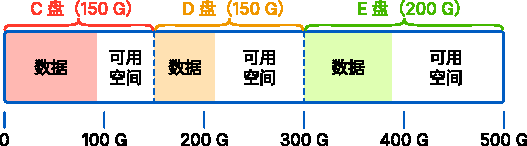
\includegraphics[width=.9\textwidth]{assets/advanced/Disk_partitions.pdf}
  \caption{分区中的数据}
  \label{fig:Disk_partitions}
\end{figure}

这种结构决定了分区可以在尾部无损进行空间调节。例如,我们可以在一个分区尾部「切」出一个新的分区(请参见\chapref{cha:new-laptop-setup}),也可以删除一个分区并把它的空间合并给前一个分区。这些操作都可以使用 Windows 自带的「磁盘管理」工具来完成。

然而,如果我们想把一个分区的空间挪给另一个分区,问题就会变得复杂起来。在上面的例子中,如果我们想把 E 盘的一部分空间转移到 D 盘,我们得先把 E 盘的数据向后移动一段距离,这样才能给 D 盘留出向后扩展的空间。

\begin{figure}[htb!]
  \centering
  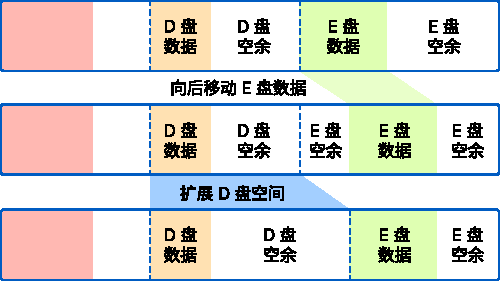
\includegraphics[width=.85\textwidth]{assets/advanced/Move_space_from_partition_to_partition.pdf}
  \caption{在分区之间转移空间}
  \label{fig:Move_space_from_partition_to_partition}
\end{figure}

如果我们需要把 E 盘的空间转移给 C 盘,就需要更复杂的数据移动,逐级将可利用的空闲空间向前转移。Windows 自带的磁盘管理无法进行这些复杂的操作,所以我们需要借助一些第三方工具来完成这个任务。下面我们隆重介绍 DiskGenius。

\subsection{用 DiskGenius 进行高级分区调整}

DiskGenius 是一款多功能磁盘管理软件,可以进行自由分区、磁盘迁移等操作(其实它还支持数据恢复,不过免费版不提供)。它有免费版,以及付费的标准版和专业版三种版本,不过我们普通用户所需的功能,免费版就已经全部包含在内了。免费版可以前往它的官网下载页面 \url{https://www.diskgenius.cn/download.php} 下载。

值得一提的是,DiskGenius 的启动画面上也会写有本章开头的「八字真言」,再一次提醒我们「数据无价」这不争的事实,也提醒我们自己的数据一定要做好备份,尤其是在这样需要对硬件进行危险的操作之前。

\begin{figure}[htb!]
  \centering
  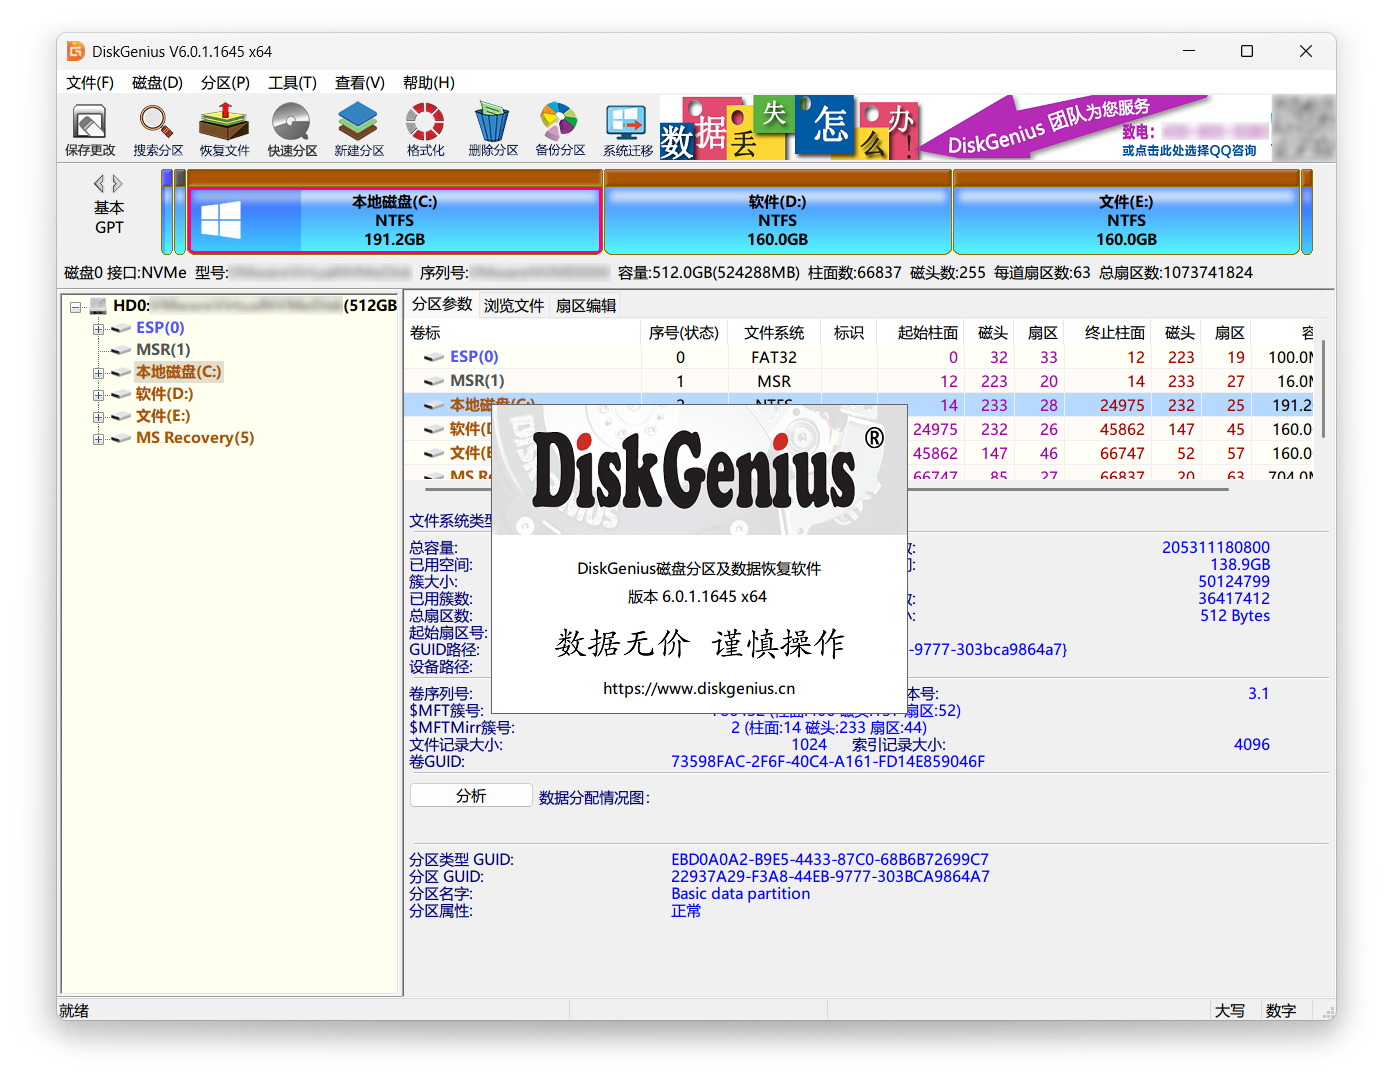
\includegraphics[width=.7\textwidth]{assets/advanced/DiskGenius.png}
  \caption{DiskGenius}
  \label{fig:DiskGenius}
\end{figure}

打开 DiskGenius,你电脑上所有的磁盘信息均会映入眼帘:左侧是你所有磁盘与分区的列表,上方有当前磁盘的使用情况,中间一大块则是选中分区的信息。想要操作某个分区,就再上方选中那个分区,点击右键即可。

\begin{figure}[htb!]
  \centering
  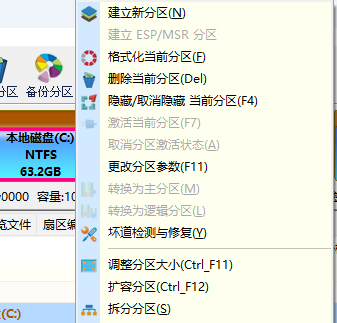
\includegraphics[width=.5\textwidth]{assets/advanced/Part_Operation.png}
  \caption{DiskGenius 的分区操作}
  \label{fig:Part_Operation}
\end{figure}

现在我们的分区结构是:C 盘、D 盘(一个很小的分区)、以及一片 30 GB 的空闲空间。现在,让我们来尝试将之前那磁盘尾部的 30 GB 空间分给在中间的 C 盘。
为了实现这样的操作,我们需要将 D 盘数据后移,把空闲空间移到 C 盘后面,再将 C 盘向后扩大。

右击空闲区域之前的那一个小分区,选择【调整分区大小】,接着,软件会弹出这样的界面:

\begin{figure}[htb!]
  \centering
  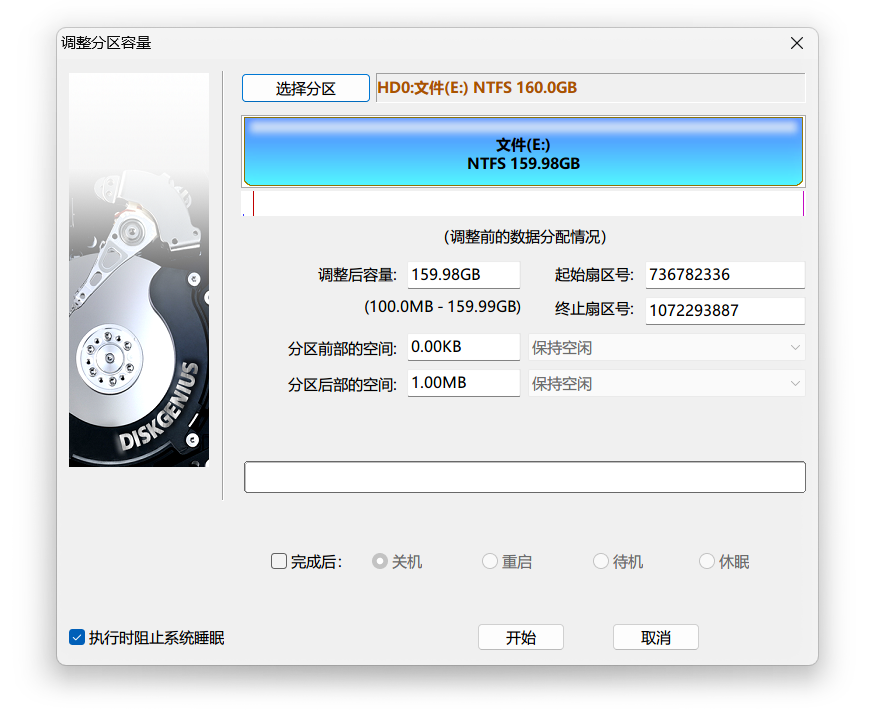
\includegraphics[width=.7\textwidth]{assets/advanced/Adjust_Part.png}
  \caption{操作分区}
  \label{fig:Adjust_Part}
\end{figure}

上方的条条是选中的分区与它周围空闲空间的情况,下面是此次调整的详细参数。你可以选择在上面的条条中直接操作,也可以选择在底下的参数中做精细调整。如果你要删除某个分区,记得先把里面的所有文件移出来或做备份。

但这次我们的任务只是想把这个小分区移到末尾去,直接在上方条条中将这个小分区拖到末尾即可(注意鼠标光标的形状,别把分区拉大了)。如果想要指定分区的容量,最好还是在底下的参数中直接输入你想要的数值。

\begin{figure}[htb!]
  \centering
  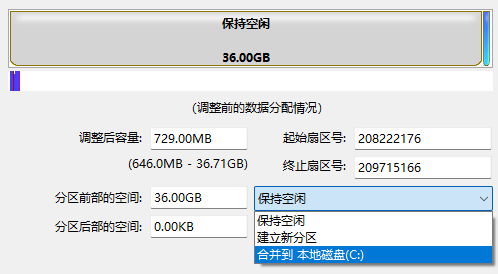
\includegraphics[width=.5\textwidth]{assets/advanced/Merge_To_C.png}
  \caption{将空余空间合并到 C 盘}
  \label{fig:Merge_To_C}
\end{figure}

拖过去之后,下方「分区前部的空间」右侧下拉框就有用了,在这里选择【合并到 本地磁盘(C:)】,然后点击【开始】,点两下【是】。\regcolor{由于我们在操作 C 盘,DiskGenius 会弹出「需要重启到 Windows PE」的警告},请仔细阅读警告,按其行事,然后再点【确定】,软件将开始工作。这段时间你可以喝杯茶,看看电脑上还有没有【确定】要点。一切顺利的话,电脑重启完毕后,你就能看到一个更大的 C 盘了!

\begin{figure}[htb!]
  \centering
  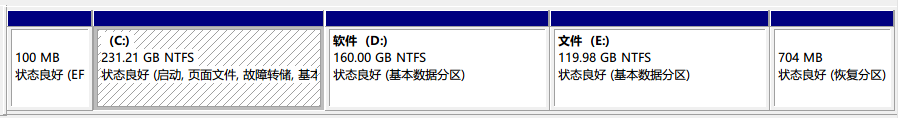
\includegraphics[width=.9\textwidth]{assets/advanced/Larger_C.png}
  \caption{更大的 C 盘}
  \label{fig:Larger_C}
\end{figure}

\begin{note}
  \regcolor{正常来说,进行分区调整是不需要重新启动的},这个例子中重启的原因是我们调整的范围涉及到 C 盘,而 C 盘上 Windows 操作系统本身正在运行,所以需要重启到一个独立的临时系统环境(即 Windows PE)中进行操作。
\end{note}

以上就是 DiskGenius 分区管理的基本使用方法。不同于只能调整分区尾部的「磁盘管理」工具,DiskGenius 不仅可以将分区向前、向后扩大或缩小,还可以移动分区在整个磁盘中的位置,是一个非常强大的磁盘管理工具。

\section{拯救「红盘」的其他方法}

进行分区调整总是存在风险的。由于上节我们已经看到,要进行分区间的空间转移,必然进行文件的移动,这就意味着有可能会出现文件损坏的情况。所以,如果你的硬盘空间不是特别紧张,我们还是建议你不要轻易进行分区调整。在这里,我们将介绍一些方法,帮助你释放硬盘空间。

\subsection{清理磁盘}

很多人在提到「清理硬盘空间」的时候总会联想到各种「卫士」「管家」中的「垃圾清理」功能,但实际上 Windows 自带了清理硬盘空间的小工具——「磁盘清理」。

在 Windows 11 中,要找到磁盘清理工具,最快的方法是按下 \keys{\Windows + S},输入「磁盘清理」,如\autoref{fig:Search_For_Disk_Clean}。打开它,选择你需要清理的分区即可。

\begin{figure}[htb!]
  \centering
  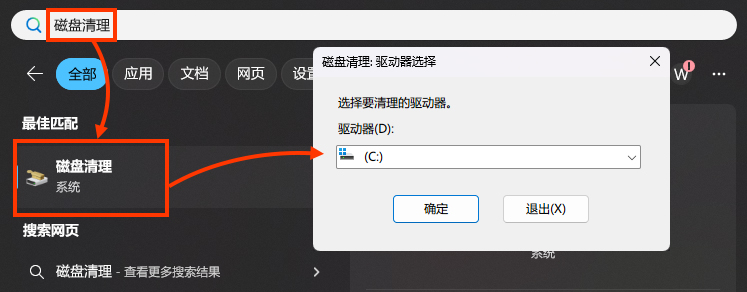
\includegraphics[width=.72\textwidth]{assets/advanced/Search_For_Disk_Clean.jpg}
  \caption{在 Windows 11 中搜索「磁盘清理」}
  \label{fig:Search_For_Disk_Clean}
\end{figure}

而在 Windows 10 中,要寻找磁盘清理工具,可以右击某个分区,点击【属性】,再点击【磁盘清理】,就可以打开清理对应分区的磁盘清理工具,如、\autoref{fig:Win_10_Disk_Clean}。

\begin{figure}[htb!]
  \centering
  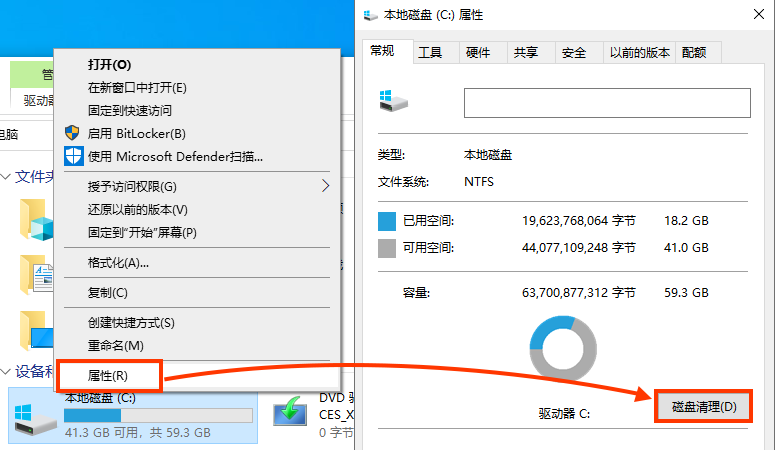
\includegraphics[width=.68\textwidth]{assets/advanced/Win_10_Disk_Clean.png}
  \caption{在 Windows 10 中寻找「磁盘清理」}
  \label{fig:Win_10_Disk_Clean}
\end{figure}

\begin{figure}[htb!]
  \centering
  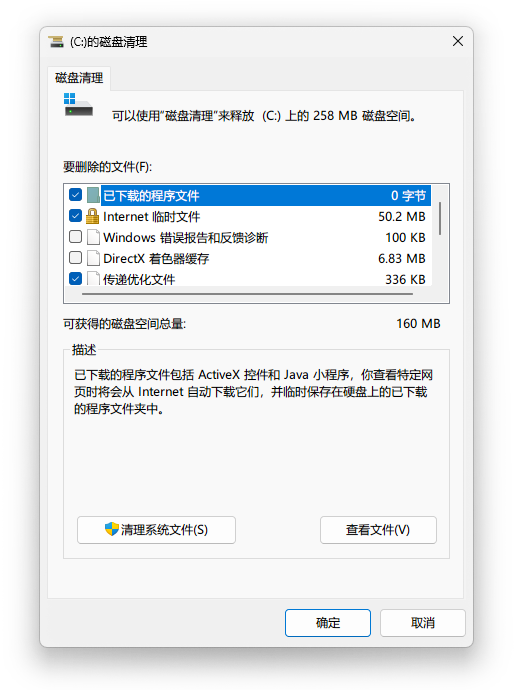
\includegraphics[width=.48\textwidth]{assets/advanced/Disk_Clean.png}
  \caption{磁盘清理工具}
  \label{fig:Disk_Clean}
\end{figure}

等待系统扫描可以清理的文件,一个窗口将会出现在屏幕上,如\autoref{fig:Disk_Clean},询问你想要清除的项目。如果你不是以管理员的权限来运行它,那么左下方会有一个「清理系统文件」的按钮,可以点击它来清理更多内容。事实上,这些地方所列出的可清理内容(包括所谓的「系统文件」)均是系统在使用过程中产生的临时文件或不那么重要的内容,如果你的空间吃紧,可以考虑全部删除。

除此之外,Windows 11 系统也可以转到系统设置→【系统】→【存储】→【清理建议】中清理系统产生的临时文件。不过要注意的是,比起「磁盘清理」工具,这里的清理内容还能包含你的「下载」文件夹。

\begin{figure}[htb!]
  \centering
  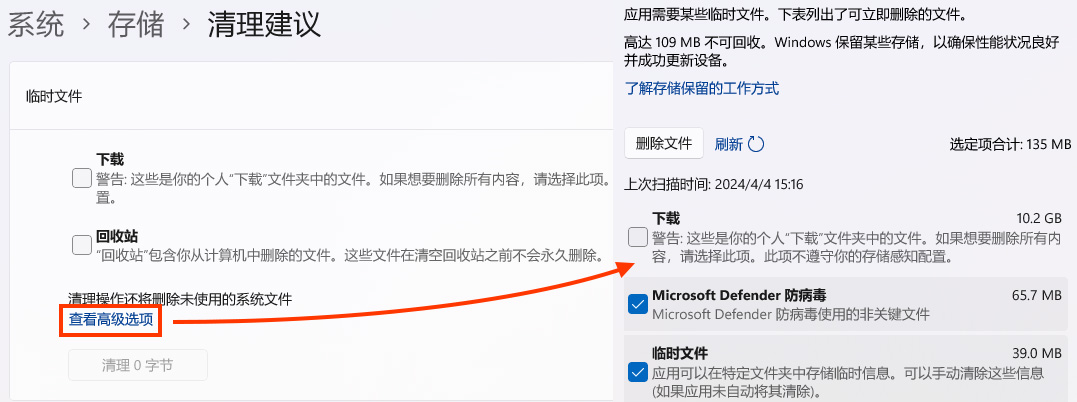
\includegraphics[width=.9\textwidth]{assets/advanced/Clean_Suggestion.jpg}
  \caption{清理建议}
  \label{fig:Clean_Suggestion}
\end{figure}

除此之外,按下 \keys{\Windows + R},输入 \MissingTT{\%temp\%}\hspace{1pt}(这也是一个环境变量)按回车,你就来到了你用户文件夹下的本地临时文件夹。如果实在没东西可删,这里的所有内容你都可以删除(不是 \MissingVerb{Temp} 文件夹本身,是它里面的所有内容),不过删除之前建议重启电脑。

但对于某些应用产生的垃圾(比如什么 QQ、微信),以及你自己用不到的个人文件,Windows 肯定无能为力了。关于这部分内容,就像我们在\chapref{cha:file-and-file-management}中说的那样——定期整理、定期打扫才是最好的方式。

\subsection{暗度陈仓 *}

怎么个「暗度陈仓」法?如果我们可以把文件/文件夹的本体移到别处有空的位置,但在原位置放上一个「链接」,让软件们都会认为这里还留着原本的文件/文件夹而照用不误,就可以在一定程度上缓解空间紧张问题了。Windows 提供的「符号链接」功能就可以帮我们实现这个目的。

符号链接可以简单地理解为一个虚拟的文件/文件夹,它指向了一个真实的文件/文件夹。例如,我可以在 \MissingVerb{C:\Missing} 下建立一个指向 \MissingVerb{D:\Chatpers} 的符号链接 \MissingVerb{C:\Missing\Chapters}。这样,对于几乎所有应用程序来说,访问 \MissingVerb{C:\Missing\Chapters} 就相当于在访问 \MissingVerb{D:\Chatpers},程序可以在其中读写文件,但实际上文件存放在 D 盘中。这样,我们就可以把一些大文件/文件夹移到其他分区,再在原位置建立符号链接,从而释放 C 盘空间。

众所周知,C 盘里的文件大都是重要的系统文件,不能轻易移动。所以\regcolor{这个办法是走投无路的选项之一},除非你非常理解你在做什么。不过说是「不能轻易移动」,但其实有一些文件夹还是可以动的。完全不能移动的有:

\begin{itemize}
  \item \MissingVerb{Windows} 文件夹:系统本体;
  \item \MissingVerb{Program} 开头的三个文件夹自身:程序文件夹的根;
  \item \MissingVerb{Users} 文件夹自身:所有用户文件夹的根。
\end{itemize}

可以移动的有:

\begin{itemize}
  \item 你的用户文件夹(不建议全移走);
  \item \MissingVerb{Program Files} 与 \MissingVerb{Program Files (x86)} 里面\regcolor{你自己装上去的程序}(不推荐,不如直接在安装的时候装到别处)。
\end{itemize}

其余的文件/文件夹均不推荐移动。也就是说,只有在实在没有办法的前提下,优先移动你用户文件夹内或前述 \MissingVerb{Local}、\MissingVerb{Roaming} 文件夹内的大型文件/文件夹。例如,Mathematica 安装的本地文档位置在 \MissingVerb{%localappdata%\Programs\Common\Wolfram Research\Documentation.zh-Hans-cn},这是一个占用空间几 GB 的文件夹,我们可以将它移到别处,譬如 \MissingVerb{F:\Link\Documentation.zh-Hans-cn},再在原位置建立同名的文件夹符号链接即可。

要建立符号链接,首先按 \keys{\Windows + S},搜索 \MissingVerb{cmd},右击【命令提示符】,选择【以管理员身份运行】。在弹出的窗口中输入下面的命令:

\begin{MissingVerbatim}[bat]
mklink /d "%localappdata%\Programs\Common\Wolfram Research\Documentation.zh-Hans-cn" "F:\Link\Documentation.zh-Hans-cn"
\end{MissingVerbatim}

其中 \MissingVerb{%localappdata%\Programs\Common\Wolfram Research\Documentation.zh-Hans-cn} 是符号链接的位置,\MissingVerb{F:\Link\Documentation.zh-Hans-cn} 是符号链接指向的位置,也就是本体的实际位置。\MissingVerb{/d} 表示「目录」,表示建立的符号链接是用于文件夹的。如果你移动的是文件而非文件夹,需要将 \MissingVerb{/d} 删掉。

但是这「暗度陈仓」的弊端也很明显。如果你一番操作下来,建立了许多符号链接,虽然这么一来 C 盘的空间压力减轻了,但是文件之间的相互关系却变得更加混乱了。如果在放置文件本体时随性而为,那只会让混乱不堪的文件指向关系更加雪上加霜。

而 Windows 没有提供从文件本体查看是否有符号链接指向它的功能,所以,我们无法知道文件本体它应当所在的原位置,也无法知道它还有没有用。更有甚者,我们可能会忘记这个文件的作用,结果误删了它。这无形之中增加了文件管理的难度。所以,如果你决定要「暗度陈仓」,请\regcolor{一定要留下必要的笔记或说明,并用一个专门的文件夹来存放符号链接的本体}。

\subsection{「治本」之道}

说真的,最能解决此类问题的方法就是加/换一块更大的硬盘,\regcolor{当上面那些方法依然解决不了那举步维艰的空间时,买一块更大的硬盘是唯一的解决方案。}

但换硬盘面临的重大问题是:旧硬盘上的内容该怎么处理。如果你换的不是系统盘,那问题不大,将数据复制粘贴即可。但如果是系统盘,那一般而言有两种方案:

\begin{itemize}
  \item 为新硬盘安装新系统,舍弃旧硬盘的系统,想办法把旧硬盘的部分数据移到新硬盘;
  \item 把原来硬盘上的所有内容原封不动地搬到新硬盘中。
\end{itemize}

如果选择前者,你需要在新硬盘上安装系统,再找出旧硬盘中你需要的文件,复制到新硬盘上。如果选择后者,则可以考虑使用 DiskGenius 的「系统迁移」功能协助你的操作。

打开 DiskGenius,选中待迁移的磁盘,在上方点击【系统迁移】,软件会弹出窗口来询问迁移的目标磁盘,选择你的新硬盘。默认情况下,DiskGenius 只会迁移与系统有关的分区,如果你的硬盘上还有别的数据分区,则需要进一步配置。

\begin{figure}[htb!]
  \centering
  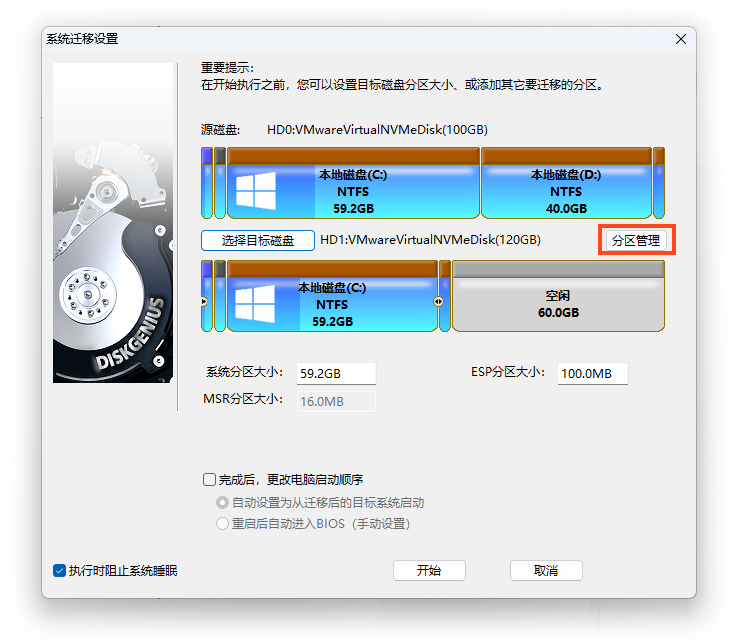
\includegraphics[width=.6\textwidth]{assets/advanced/Configure_System_Migration.png}
  \caption{配置系统迁移}
  \label{fig:Configure_System_Migration}
\end{figure}

如\autoref{fig:Configure_System_Migration} 和\autoref{fig:Select_Migrating_Partition} 所示,点击中间右侧的【分区管理】,在弹出的窗口中点击【添加分区】,选择你需要的分区,点【确定】即可添加。

\begin{figure}[htb!]
  \centering
  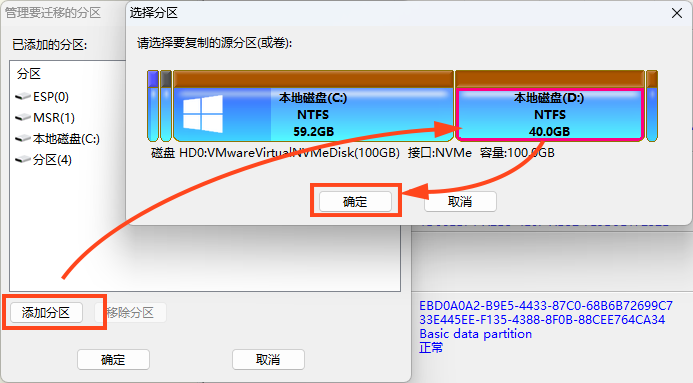
\includegraphics[width=.6\textwidth]{assets/advanced/Select_Migrating_Partition.png}
  \caption{选择要迁移的分区}
  \label{fig:Select_Migrating_Partition}
\end{figure}

回到刚才的窗口,勾选【完成后,更改电脑启动顺序】,点击【开始】,软件将会询问你想采用的执行方式,可以选择【热迁移】,它会立即开始迁移工作,不过我们不建议这时还运行别的程序。这时你可以喝杯茶,等待软件完成工作,然后重启电脑。重启之后,你会发现现在的系统已经位于刚刚换上来的那块硬盘了,而原来的硬盘你可以选择格式化,让它来做点别的事情。

\begin{figure}[htb!]
  \centering
  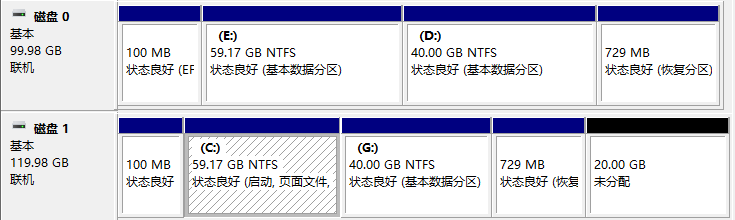
\includegraphics[width=.75\textwidth]{assets/advanced/Migration_Result.png}
  \caption{迁移结果}
  \label{fig:Migration_Result}
\end{figure}

\section{到底什么是文件链接 *}

上文中,我们简单介绍了「符号链接」,这是一种可以让文件/文件夹指向其他文件/文件夹的方法。其实,符号链接是「文件链接」的一种,Windows 还提供了其他类型的文件链接。本节我们将深入介绍文件链接的概念与使用方法。

在\chapref{cha:file-and-file-management}一章中我们已经介绍了「快捷方式」的基本概念,但快捷方式说到底是一个文件,一个扩展名为 \MissingVerb{lnk} 的文件。「不同类型的文件需要用不同的软件来打开」,这也是我们已经知道的,那么快捷方式呢?答案是文件资源管理器,快捷方式是作为文件资源管理器的扩展而存在的,资源管理器读取它,就知道该去哪里找文件。

不妨试一试用记事本来打开一个快捷方式\footnote{直接在记事本里面点【打开】是不行的,因为「打开」操作调用了文件资源管理器。}:

\begin{itemize}
  \item 在桌面按住 \keys{Shift} 点右键,选择【在此处打开 PowerShell 窗口】;
  \item 先输入 \MissingVerb{dir},按回车,你就可以看到目前你桌面上的所有文件与文件夹;
  \item 再挑一个快捷方式,输入 \MissingVerb{notepad <快捷方式(带扩展名)>},按回车,你就会看到你选的快捷方式的「真面目」。
\end{itemize}

那么有没有一种「更强力的快捷方式」,让无论是哪个应用都知道去找目标文件呢?这就是文件链接。文件链接有两种类型——「硬链接」与「符号链接」(又称「软链接」),让我们来看看它们是个什么玩意。

\subsection{符号链接}

符号链接的行为有点像快捷方式,即一个指向其目标的「指针」,只不过,快捷方式只对资源管理器有效,而符号链接则对几乎任何软件来说都是快捷方式。既然它的行为类似快捷方式,那关于「删了它会怎么样」之类的问题想必不用多费口舌。总结起来就几句话:删除链接不会影响本体;删除本体则链接还在,但是找不到目标。

\begin{figure}[htb!]
  \centering
  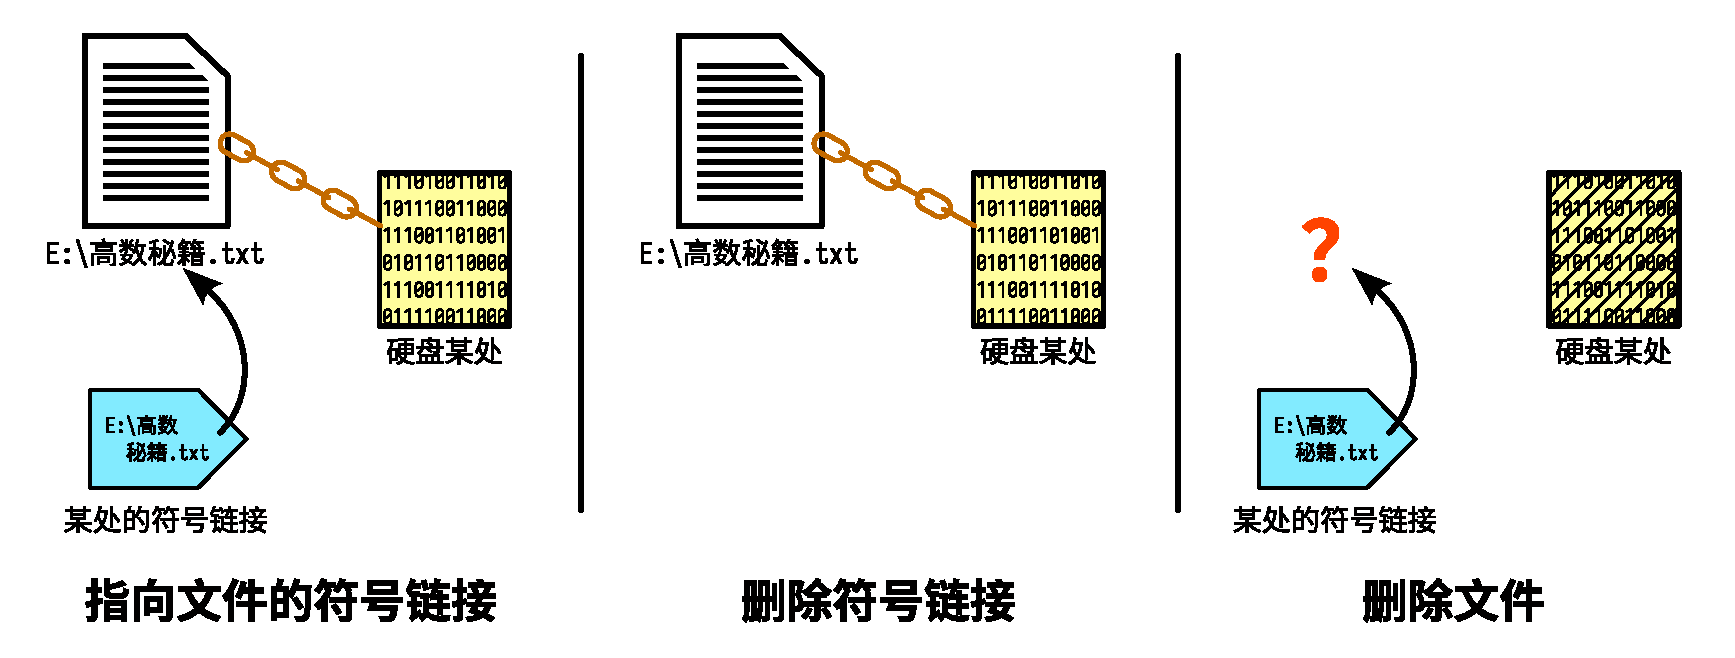
\includegraphics[width=.8\textwidth]{assets/advanced/Symbolic_Link.pdf}
  \caption{符号链接}
  \label{fig:Symbolic_Link}
\end{figure}

要想创建符号链接,你可以使用命令提示符中的 \MissingVerb{mklink} 命令或者 PowerShell 中的 \MissingVerb{New-Item} 命令。这两种方法各有优劣,需要根据实际情况来决定使用哪一种。欲使用 \MissingVerb{mklink},按照以下步骤来:

\begin{enumerate}
  \item 按下 \keys{\Windows + R},输入 \MissingVerb{cmd} 并回车以打开命令提示符窗口;
  \item 如果你的目标是一个文件,请使用如下语法:
    \begin{MissingVerbatim}[bat]
      mklink <链接所在路径> <本体所在路径>
    \end{MissingVerbatim}
    如果是文件夹,则需指定 \MissingVerb{/d} 选项,即:
    \begin{MissingVerbatim}[bat]
      mklink /d <链接所在路径> <本体所在路径>
    \end{MissingVerbatim}
    此前提到的 \MissingVerb 这样的环境变量也可以使用,带空格的路径记得打上双引号。
\end{enumerate}

欲使用 \MissingTT{New-Item}(简写为 \MissingVerb{ni}),按照以下步骤来:

\begin{enumerate}
  \item 按下 \keys{\Windows + X},选择【PowerShell】或【终端】;
  \item 使用如下语法创建符号链接:
    \begin{MissingVerbatim}[pwsh]
      ni <链接所在路径> -i SymbolicLink -ta <本体所在路径>
    \end{MissingVerbatim}
    这种方式对文件与文件夹都有效,但 PowerShell 无法识别 \MissingVerb 这样的环境变量。同样,带空格的路径记得打上双引号。
\end{enumerate}

看上去 \MissingVerb{New-Item} 可以用一个命令搞定文件与文件夹,挺通用,但目前它有一个重大问题——无法处理带西文方括号(「\MissingVerb{[}」和「\MissingVerb{]}」)的路径。所以\regcolor{如果有路径包含了西文方括号,请使用 \MissingTT{mklink}}。如果提示什么「权限不足」之类的信息,请用管理员权限再试一次。

实际上,在创建符号链接的时候,不需要让两者的名称一致,例如你可以创建一个名为 \MissingVerb{大物教程} 的链接,但它指向你的 \MissingVerb{高数秘籍.txt}。然而,若是这样做,虽然文件资源管理器知道它指向的是个什么东西,也知道用什么软件来打开目标,但其他应用可就不一定了。故我们\regcolor{推荐创建链接时使用与目标完全一致的名称}。

\subsection{硬链接}

硬链接的作用,一言以蔽之——从多个位置访问、修改磁盘上同一块内容。看起来好像和符号链接没差多少,但,请看下图。

\begin{figure}[htb!]
  \centering
  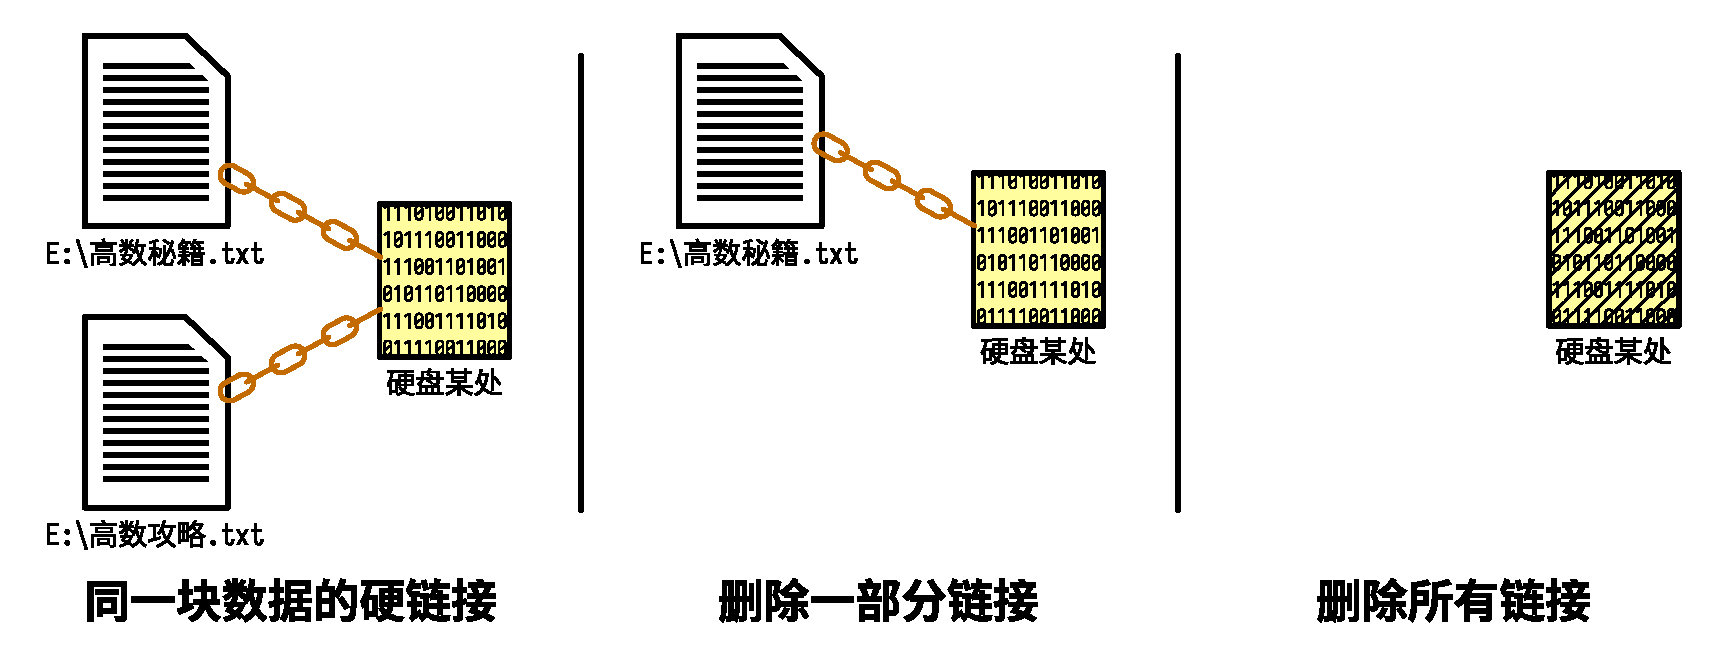
\includegraphics[width=.8\textwidth]{assets/advanced/Hard_Link.pdf}
  \caption{硬链接}
  \label{fig:Hard_Link}
\end{figure}

以一个文件为目标建立硬链接,其实是与目标文件对应的硬盘数据相连接。从某种意义上而言,这些连接到同一块数据的不同文件,彼此之间都是硬链接关系。这样一来,如果我们打开其中一个文件做修改,这实际上是通过其中一个文件修改了硬盘数据,那么再打开其他硬链接的文件,我们会发现内容是我们刚刚修改过的。譬如上图中,给 \MissingVerb{E:\高数秘籍.txt} 加一句话,那么查看 \MissingVerb{E:\高数攻略.txt} 则会发现也多了一句完全一样的话。但若删除一部分链接(例如删除 \MissingVerb{E:\高数攻略.txt}),只要这块数据仍存有链接,那么它就不会被真正删除。也就是说,要想删除硬链接过的文件,需要删除链接到同块数据的所有文件。

要想建立硬链接,同样是使用 \MissingVerb{mklink} 或者 \MissingVerb{New-Item} 命令。然而,由于绑定了磁盘上的数据,\regcolor{硬链接无法跨磁盘分区建立}。欲使用 \MissingVerb{mklink},按照以下步骤来:

\begin{enumerate}
  \item 按下 \keys{\Windows + R},输入 \MissingVerb{cmd} 并回车,打开命令提示符窗口;
  \item 如果目标是一个文件,请使用如下语法:
    \begin{MissingVerbatim}[bat]
      mklink /h <链接所在路径> <本体所在路径>
    \end{MissingVerbatim}
    如果是文件夹,则需附加指定 \MissingVerb{/d} 选项,即:
    \begin{MissingVerbatim}[bat]
      mklink /h /d <链接所在路径> <本体所在路径>
    \end{MissingVerbatim}
    带空格的路径记得打上双引号。
\end{enumerate}

欲使用 \MissingVerb{New-Item},按照以下步骤来:

\begin{enumerate}
  \item 按下 \keys{\Windows + X},选择【PowerShell】或【终端】;
  \item 使用如下语法创建符号链接:
    \begin{MissingVerbatim}[pwsh]
      ni <链接所在路径> -i HardLink -ta <本体所在路径>
    \end{MissingVerbatim}
    它对文件与文件夹都有效,但也无法处理带西文方括号的路径,无法识别环境变量。当然,带空格的路径记得打上双引号。
\end{enumerate}

按照硬链接的行为,\regcolor{无论一份数据有多少硬链接,磁盘上都应该只有一份文件的数据,只占一份文件的空间}。事实的确如此,但文件资源管理器不这么想——有多少链接,它就给你算多少份文件大小,于是乎,就有了这样占用空间比整个硬盘还大的奇景:

\begin{figure}[htb!]
  \centering
  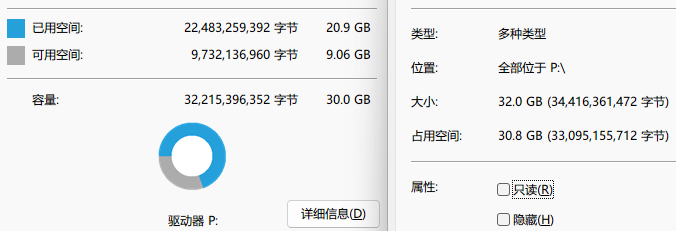
\includegraphics[width=.8\textwidth]{assets/advanced/Interesting_Storage_Size.png}
  \caption{奇怪的占用空间}
  \label{fig:Interesting_Storage_Size}
\end{figure}

\subsection{目录联接}

如果你看到过 \MissingVerb{mklink} 的语法说明(没看到的可以现在看看,执行 \MissingVerb{mklink} 就行),你可能会发现在指定链接类型时,除了指定文件夹的 \MissingVerb{/d} 与指定硬链接的 \MissingVerb{/h} 选项以外,居然还有一个 \MissingVerb{/j} 选项,按底下的说明,它是「目录联接」。

目录联接其实类似于文件夹符号链接,要是只用在自己电脑的文件上,那就没什么两样,但要是通过网络访问其他电脑上的文件,那就有差别了。

假定有 Reimu 和 Marisa 两台电脑,二者之间通过网络共享数据,即它们的路径分别为 \MissingVerb{\\Reimu} 与 \MissingVerb{\\Marisa}。Reimu 有一个文件夹,本地路径是 \MissingVerb{C:\Folder},除此之外还有一个文件夹符号链接 \MissingVerb{C:\SymLink} 与一个目录联接 \MissingVerb{C:\Junc},它们均指向 \MissingVerb{C:\Folder}。现在 Marisa 要通过网络来访问这个符号链接与目录联接,则 Reimu 那边的目录联接对 Marisa 来说的路径是 \MissingVerb{\\Reimu\C$\Junc},指向了 \MissingVerb{\\Reimu\C$\Folder}——正确的位置;但是,符号链接的路径是 \MissingVerb{\\Reimu\C$\SymLink},却指向了 \MissingVerb{\\Marisa\C$\Folder}——Marisa 自己这边的位置!

这告诉我们,符号链接并不会循着网络位置来寻找目标,而只是在本地寻找。故若需要为网络访问为目的制作链接,请使用目录联接。

\practice

\begin{enumerate}
  \item 将一个文件/文件夹移到别处,再在原位置建立符号链接、硬链接及快捷方式,照常使用、访问它,看看三者有什么不同。
  \item 尝试用「磁盘清理」工具清一下你的所有分区。
  \item 查看你电脑上的分区情况,以及是否存在细小的未分配空间,若有必要,可以试着重新分区。(记得备份数据!)
\end{enumerate}